\chapter{Objetos y Fenómenos Astrofísicos Relevantes}
\section{Nubes Moleculares Gigantes}

Las grandes ``guarderías'' de estrellas a lo largo de la Galaxia se localizan en nubes moleculares gigantes, compuestas principalmente por hidrógeno molecular $\mathrm{H_2}$.
Siendo que esta molécula solo emite radiación en ultravioleta, donde el medio interestelar tiene una alta extinción, para detectar la presencia de las nubes moleculares se recurre a otras moléculas llamadas ``trazadoras'', principalmente $\mathrm{CO}$, la segunda molécula más abundante en el medio interestelar, que posee líneas espectrales en el rango de las ondas de radio.

Complejos aomo el de Taurus-Auriga se formaron debido a la convergencia de dos flujos de material neutro \citep{Ballesteros:1999} que se enfrió y se volvió más denso debido a inestabilidades térmicas \citep{Hennebelle:1999}. Muchas de estas nubes moleculares tienen forma filamentaria debido a que se están colapsando gravitacionalmente en caida libre \citep{Ballesteros:2011}. Dentro de los filamentos puede haber colapsos locales que pueden dar lugar a regiones de formación estelar de baja masa o incluso asociaciones OB como es el caso de la Nebulosa de Orión \citep{Hartmann:2007}.

\section{La Nebulosa de Orión}

\begin{figure*}
    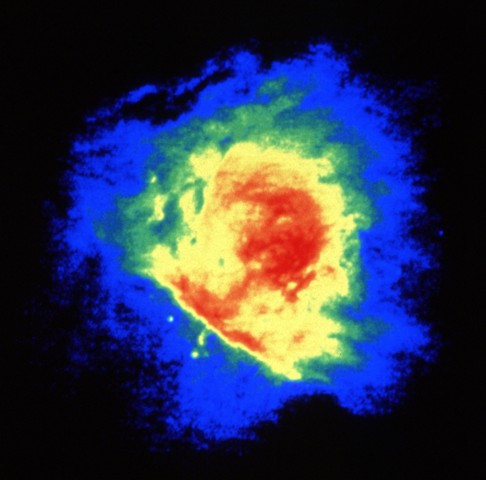
\includegraphics[width=0.5\linewidth]{./Figures/OrionVR13A} 
  \caption{La Nebulosa de Orión observada por el VLA en la banda L ($\lambda = \SI{20}{cm}$, $\nu = \SI{1.4}{GHz}$, \citet{Yusef:1990}).}
\end{figure*}

La Nebulosa de Orión (ONC por sus siglas en inglés), ubicada a $\sim \SI{414}{pc}$ \citep{Menten:2007}, es probablemente la región HII mejor estudiada del cielo (ver \S \ref{sec:HII}). Forma parte de la nube molecular gigante de Orión, de donde se distinguen dos sub-unidades, llamadas Orión A y Orión B. ONC forma parte de Orión A. El cúmulo de estrellas que se formó y que es responsable de la región \Ion{H}{II} se conoce como asociación OB Ori Id, cuyos miembros más prominentes son un grupo de cuatro estrellas conocidas como el ``Trapecio''. La más masiva de éstas es \thC{}, de clasificación espectral O6 aproximadamente (ver tabla ), tiene una luminosidad de \SI{4e5}{L_\odot} y una temperatura de \SI{4e-4}{K}. Cuando la región HII se encuentra embebida en el gas molecular, la región \Ion{H}{II} no puede ser visible en el rango óptico del espectro.  En el caso de ONC, que se ubica cerca del borde de la nube molecular Orion A, el gas ionizado caliente, que posee una presión mayor que el gas molecular frío, se escapa hacia el gas adyacente a la nube molecular en forma de ``flujo de champaña'' (figura \ref{fig:champagne}), y de esta manera el gas ionizado puede ser visible por medio de diferentes líneas espectrales, tanto de hidrógeno como de otros elementos. 

\begin{figure}
  \begin{tabular}{lr}
    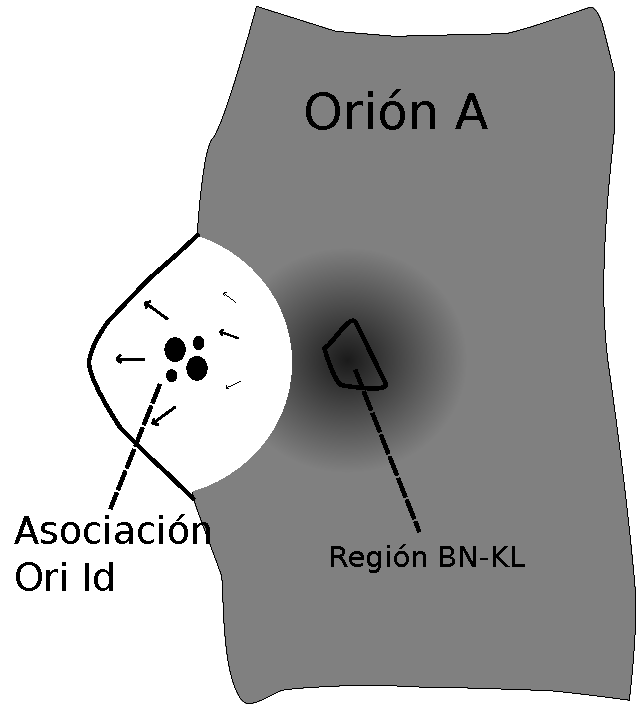
\includegraphics[width=0.4\linewidth]{./Figures/champagne} &
    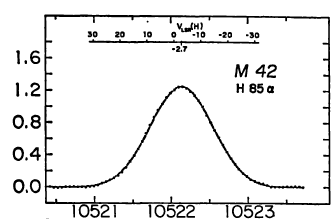
\includegraphics[width=0.5\linewidth]{./Figures/H85-alpha}
    \end{tabular}
  \caption{Izquierda:Representación esquemática de la Asociación Ori Id y su ubicación dentro de la nube molecular gigante Orión A. La región BN-KL es una región de formación estelar muy activa donde se observan entre otras cosas, máseres de agua y SiO y flujos moleculares \citep{Stahler:2004}. Derecha: Línea espectral $H~85~\alpha$ de hidrógeno de ONC. El eje horizontal corresponde a la frecuencia en MHz, mientras que el eje verical representa la temperatura de antena. El espectro muestra un corrimiento al azul que muesta que el gas se acerca a una velocidad de $\sim 3\mathrm{~km~s^{-1}}$ \citep{Stahler:2004, Churchwell:1970}}
  \label{fig:champagne}
\end{figure}


%\section{Estrellas ``Errantes''}
%\section{Discos Protoplanetarios}
%\subsection{Formación}

\section{Proplyds}
\subsection{Descubrimiento}
Observaciones en óptico de la región del trapecio en filtros de banda angosta de diferentes líneas de emisión tales como \Ion{H}{\alpha}, \Ion{H}{\beta}, [\Ion{O}{III}], [\Ion{N}{II}], [\Ion{S}{II}] y continuo, revelaron la existencia de objetos puntuales únicamente visibles en líneas de alta ionización (\Ion{H}{\alpha}, \Ion{H}{\beta} y [\Ion{O}{III}]) que fueron inicialmente denominados como ``condensaciones nebulares'' \citep{Laques:1979}. Hasta el momento no se sabía con certeza si ``condensaciones nebulares'' eran en realidad condensaciones nebulares (regiones donde la densidad de la nebulosa es inusualmente alta por alguna razón o bien esferas de gas molecular cuya envolvente fue ionizada y que la radiación de la estrella central la está ``erosionando'') o si se trataba de protoestrellas de baja masa cuyo disco protoplanetario estaba siendo fotoevaporado por la estrella central \citep{churchwell:1987}. No fue sino hasta que se contó con observaciones de alta resolución con el Telescopio Espacial Hubble (HST) que se se pudo determinar la verdadera naturaleza de estos objetos \citep{ODell:1993} y la razón por la que se les denominó ``proplyds'' (PROtoPLanetarY DiskS). A su vez se encontraron por primera vez arcos delgados y otras estructuras de gran interés.

\subsection{¿Qué es un proplyd? Breve introducción \citep{Johnstone:1998}}

Las imágenes del HST de la Nebulosa de Orión mostraron imágenes de discos alrededor de estrellas jóvenes de baja masa. Algnuos se ven como siluetas oscuras que contrastan con la nebulosa, y otros casos son visibles en líneas de emisión de líneas de alta ionización. Un proplyd típico tiene forma cometaria, con una cabeza brillante que apunta hacia la fuente de radiación ionizante, y una cola que se extiende en dirección contraria a ésta. La explicación a esta forma es que el disco protoplanetario está siendo fotoevaporado por la radiación ionizante de una estrella masiva (\thC{} en caso de la Nebulosa de Orión), la cabeza es un frente de ionización cuyo radio escala como $R_{IF} \propto D^{2/3}$, donde $D$ es la distancia a la estrella masiva. La forma de la cola se debe a radiación ionizante difusa, producto de dispersión por polvo y por recombinaciones (Figura \ref{fig:prop-shape}). \citet{churchwell:1987} ya había notado que la tasa de pérdida de masa observada
en el gas ionizado implicaba que la fuente de este gas debía oscurecer a la protoestrella huésped, a menos que proviniera de un disco circumestelar. De la
emisión de radio observada, se estima la densidad electrónica en $n_e \sim \SI{e6}{cm^{-3}}$ y la tasa de pérdida de masa en $\dot{M} \sim \SI{e-7}{M_\odot.yr^{-1}}$.

\begin{figure}
  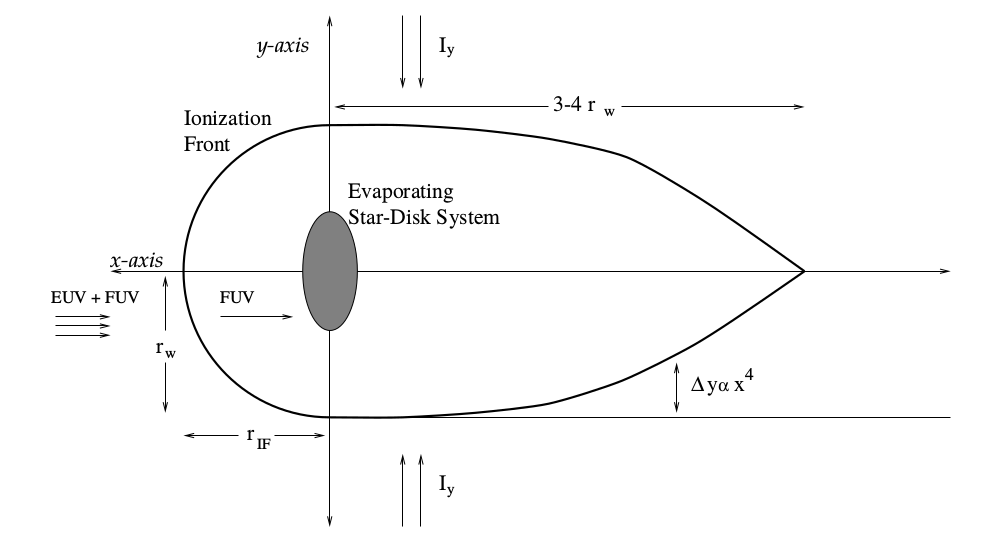
\includegraphics[width=0.8\linewidth]{./Figures/Johnstone-shape}
  \caption{Representación esquemática de la formación de un frente de ionización hemisférico y de una cola de gas ionizado detrás del disco en proceso de fotoevaporación. $r_{IF}$ y $r_w$ representan el radio del frente de ionización en las direcciones de los ejes $x$ e $y$, respectivamente. $I_y$ representa el campo de radiación difusa. Por detrás del disco, la radiación difusa calienta el gas del disco provocando otro flujo fotoevaporado. $\Delta y$ es la diferencia entre la forma actual del frente de ionización por detrás del disco y una forma cilíndrica. La forma de la colase explica como que el flujo de radiación $I_y$ es capaz de penetrar más cerca del eje $x$ conforme uno se aleja del disco, donde el flujo fotoevaporado es menos denso.}
    \label{fig:prop-shape}
\end{figure}


\subsection{Mecanismos de fotoevaporación \citep{Johnstone:1998}}

El principal mecanismo de fotoevaporación es el campo de radiación de la estrella central, en la parte ultravioleta del espectro electromagnético. Según la masa de la estrella central, podemos tener dos clases de flujo radiativo: Dominado por el ultravioleta lejano (FUV, $h\nu < \SI{13.6}{eV}$) o dominado por el ultravioleta extremo (EUV, $h\nu \geq \SI{13.6}{eV}$). En general, el FUV se encarga de disociar moléculas y de calentar el gas de la región de fotodisociación (PDR) hasta temperaturas de 100 - 1000 K, mientras que el EUV puede ionizar el gas y elevar su temperatura hasta \SI{e4}{K}. El EUV no puede atravesar el frente de ionización (IF) pero el FUV sí.

En el caso de que el flujo sea dominado por el EUV, la presión térmica del flujo fotoevaporado es determinada por la fotoionización, la PDR producida por el FUV es delgada. El gas calentado por el FUV se mueve de manera subsónica hasta llegar al IF y la tasa de pérdida de masa depende de la tasa de ionización inducida por el EUV.

Si el flujo está dominado por el FUV, la presión térmica depende del calentamiento por el FUV. El gas tibio se expande como un viento que empuja el IF lejos del disco. La tasa de pérdida de masa la determina la temperatura de la PDR, el flujo FUV y la opacidad del polvo a las longitudes de onda del FUV. Inicialmente la forma del disco impone una geometría cilíndrica en el flujo fotoevaporado, pero eventualmente los gradiente de presión tornan esta geometría en esférica.

Las ecuaciones de continuidad de la masa y el momento restringen la velocidad del flujo neutro antes de alcanzar el IF. Mas allá de éste, la presión del gas hace que éste se expanda a velocidades del orden de una a dos veces la velocidad del sonido. Para el gas neutro dentro del IF hay dos posibles soluciones: si el gas neutro es supersónico entonces el IF será de baja densidad (Tipo R) con bajo contraste de densidad entre gas neutro y gas ionizado. O si el gas neutro es subsónico se formará un IF tipo D con un gran contraste de densidad entre el gas neutro y el gas ionizado. Sin embargo, sin importar qué tipo de radiación domina la fotoevaporación, el gas neutro permanece a velocidades subsónicas al llegar al IF, por lo que dicho frente será tipo D. En el caso de un flujo dominado por el EUV, el gas neutro permanece a velocidad subsónica, su velocidad decae como $v_I \propto r^{-2}$ y llega a \SI{0.5}{km.s^{-1}} al llegar al frente de ionización. Cundo el flujo es dominado por el FUV, el gas neutro se acelera hasta llegar a velocidades supersónicas, luego atraviesa un choque isotérmico que lo desacelera y llega al frente de ionizacion a \SI{0.5}{km.s^{-1}}.

  \begin{figure}
    \begin{tabular}{cc}
      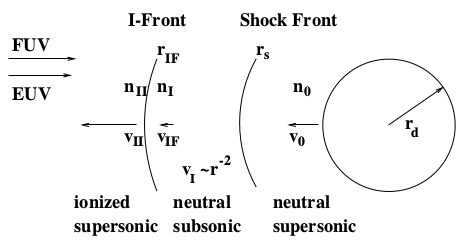
\includegraphics[width=0.5\linewidth]{./Figures/Johnstone-2} &
      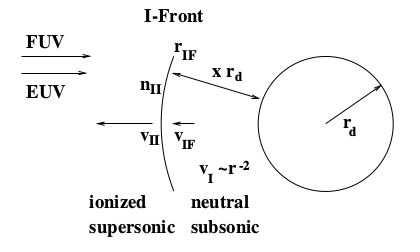
\includegraphics[width=0.5\linewidth]{./Figures/Johnstone-3}
    \end{tabular}
    \label{fig:EUV-FUV-IF}
    \caption{Representación esquemática de las regiones del flujo fotoevaporado de un proplyd. Izquierda: Cuando el flujo es dominado por el FUV. Derecha: Flujo dominado por EUV \citep{Johnstone:1998}}
  \end{figure}
  

Sin importar el tipo de mecanismo de fotoevaporación dominante, el flujo fotoevaporado solo si la presión térmica supera a la gravedad de la protoestrella. Entonces, el flujo fotoevaporado solo existe a partir de un radio crítico $r_g$, donde este radio se estima a partir del balance entre la energía necesaria para escapar de una órbita kepleriana y la energía térmica:
\begin{align}
  r_g = \frac{GM_*}{a^2}
\end{align}
Donde $M_*$ es la masa de la protoestrella y $a$ es la velocidad del sonido del gas. Para las protoestrellas típicas del trapecio la masa típica es de
$M_* = 0.2~M_\odot$. Para el gas neutro la velocidad del sonido es de $a_I \sim \SI{3}{km.s^{-1}}$ y para el gas ionizado es de $a_{II} \sim \SI{10}{km.s^{-1}}$.
Por tanto, el radio gravitacional para un flujo dominado por el EUV es de $r_{gII} \sim \SI{2}{AU}$ y para un flujo dominado por el FUV es de $r_{gI} \sim \SI{20}{AU}$.
\section{Objetos LL}
\subsection{Mapa de Objetos}
%\section{Vientos Estelares}

\includegraphics[width=0.1\linewidth]{./Figures/tux-development}
\section{Regiones HII \citep{Stahler:2004}}
\label{sec:HII}
\newcommand\Nio{\ensuremath{\mathcal{N}}}
%\newcommand\N{\ensuremath{\mathcal{N}}}

Consideremos el caso en que se forma una estrella masiva dentro de una nube molecular, que por simplicidad está compuesta exclusivamente de hidrógeno molecular $\mathrm{H_2}$. La estrella masiva emite fotones ultravioleta que tienen la energía suficiente para disociar el $\mathrm{H_2}$  como para ionizar el hidrógeno atómico resultante. Luego el plasma ionizado se recombina para volver a ser \Ion{H}{I} emitiendo líneas espectrales de diversas energías, siendo la más energética la línea de \Ion{Ly}{\alpha}. Como al realizar una ionización se pierde un fotón ionizante y el flujo de radiación proveniente de la estrella es finito, entonces la estrella solo puede ionizar la región de la nube más próxima a ésta. Si suponemos que la nube tiene densidad uniforme, entonces esta región tendrá forma esférica, conocida como \textit{esfera de Strömgren}.

\subsection{Esfera de Strömgren}

El plasma ionizado dentro de la Esfera de Strömgren se encuentra en balance de ionización, esto es, que la tasas de ionización y la de recombinación son iguales. La tasa de ionizaciones es igual a la cantidad de fotones ionizantes que emite la estrella central por segundo. Esto es, los fotones que poseen una energía mayor al límite de Lymann, que corresponde a  $E = \SI{13.6}{eV}$, o bien $\lambda = \SI{912}{\angstrom}$. En la tabla \ref{tab:ionizing-radiation} se muestra la tasa de fotones ionizantes $\Nio_*$ para estrellas masivas de tipo espectral O y B temprano.

\begin{table}
  \begin{tabular}{cccc} \hline 
    Tipo & Masa & $\log \Nio_*$ & $\log \Nio_{FUV}$ \\
    Espectral & (\SI{}{M_\odot}) & (\SI{}{s^{-1}}) & (\SI{}{s^{-1}})  \\
    \hline
    O4 & 70 & 49.9 & 49.5 \\
    O5 & 60 & 49.4 & 49.2 \\
    O6 & 40 & 48.8 & 48.8 \\
    O7 & 30 & 48.5 & 48.6 \\
    O8 & 23 & 48.2 & 48.4 \\
    O9 & 20 & 47.8 & 48.2 \\
    B0 & 18 & 47.1 & 48.1 \\
    B1 & 13 & 45.4 & 47.5 \\
    B2 & 10 & 44.8 & 47.1 \\
    \hline
  \end{tabular}
  \caption{Tasa de fotones ionizantes para estrellas masivas \citep{Stahler:2004}}
  \label{tab:ionizing-radiation}
\end{table}

El radio de esta esfera se denomina \textit{Radio de Strömgren} que viene dado por:

%Por otro lado, la tasa volumétrica de recombinaciones se escribe como:

%\begin{align}
%  \ensuremath{\mathcal{R}} = n_e n_p \alpha_{rec}(T) = n^2_e \alpha_{rec}(T)
%\end{align}

%Donde $\alpha_{rec}$ es el \textit{coeficiente de recombinación}, y es una función solo de la temperatura. La última iguladad se obtiene asumiendo neutralidad de la carga.

%La tasa total de recombinaciones se obtiene integrando $\ensuremath{\mathcal{R}}$ en el volumen de la región $HII$, asumiendo que tanto la densidad de electrones como la tempertaura son constantes espacialmente. De esta manera la condición de balance de ionización queda como sigue:

%\begin{align}
%  \Nio_* = \frac{4\pi}{3} n^2_e \alpha'_{rec}(T)R^3_s 
%\end{align}

%Donde $R_s$ es el \textit{radio de Strömgren}. Es importante notar que el coeficiente de recombinación primado es diferente del coeficiente no primado: el coeficiente de recombinación primado no toma en cuenta las recombinaciones al nivel $n = 1$ debido a que estas recombinaciones producen fotones de $E = 13.6\mathrm{~eV}$ que son capaces de ionizar el hidrógeno neutro.

%Como la densidad de la nube original no cambia apreciablemente cuando el gas es ionizado debido a que el tiempo en que esto pasa es muy corto (como mostraremos en la siguiente sección), entonces $n_e = n^0_H$, donde $n^0_H$ es la densidad de $HI$ en la región contigua a la nube, y a su vez $n^0_H = n_{H_2}$, donde $n_{H_2}$ es la densidad de gas molecular. Con esto podemos calcular el radio de Strömgren como sigue:

\begin{align}
  R_s = \left[\frac{3\Nio_*}{4\pi\alpha'_{rec}(n^0_H)^2}\right]^{1/3} = 0.4\mathrm{~pc}\left(\frac{\Nio_*}{10^{49}\mathrm{~s^{-1}}}\right)^{1/3}\left(n_{H_2}\right)^{-2/3} \label{eq:stromgren}
\end{align}

Donde $\alpha'_{rec}$ es el coeficiente de recombinación a todos los niveles energéticos del hidrógeno excepto el estado base, $n^0_H$ y $n_{H_2}$ son la densidad numérica del hidrógeno neutro y del hidrógeno molecular donde está embebida la región HII, respectivamente.

En la expresión numérica, se adopta una temperatura de $10^4\mathrm{~K}$ que es la temperatura característica de una región $HII$ y con la que el coeficiente de recombinación $\alpha'_{rec}$ adopta un valor de $2.6\times 10^{-13}\mathrm{~cm^3~s^{-1}}$.

Dentro de la región $HII$, la probabilidad por unidad de tiempo de ionizar un átomo de hidrógeno dado es mucho mayor a la probabilidad de una recombinación, por lo que el gas está casi completamente ionizado. Sin embargo, en los bordes de la región $HII$, la densidad de gas neutro aumenta debido a que en dicha región el flujo de fotones ionizantes ha sido atenuado por todo el gas ionizado más próximo a la estrella. La transición de gas ionizado a gas neutro tiene un grosor $\Delta r$ que corresponde al camino libre medio del gas neutro. Esto es:

\begin{align}
\Delta R = \frac{1}{\sigma_{\nu_1}n^0_H}  
\end{align}

Donde $\sigma_{\nu_1}$ es la sección recta de un átomo de hidrógeno en el estado base, evaluada en la longitud de onda del límite de Lymann. Utilizando $\sigma_{\nu_1} = 6.8\times 10^{-18}\mathrm{~cm^2}$ y $n^0_H = 2\times 10^{3}\mathrm{~cm^{-3}}$ obtenemos que $\Delta r = 7.4\times 10^{13}\mathrm{~cm} \sim 5\times 10^{-5}~R_s$, lo que muestra que las regiones $HII$ tienden a tener bordes bien delimitados.

\subsection{Primera y Segunda expansión}

Las esferas de Strömgren no son objetos estáticos, sino que se expanden con el tiempo. Este proceso ocurre en dos etapas: en la primera inicialmente no existe ninguna región $HII$ pero que la radiación ultravioleta de la estrella hace que se expanda rápidamente al disociar e ionizar el gas a su alrededor hasta alcanzar el radio de Strömgren. En la segunda expansión la diferencia de presiones entre el gas ionizado de la región $HII$, mucho mayor que la del gas neutro que lo rodea, provoca otra expansión más lenta que la primera hasta que haya equilibrio de presión.
%A continuación explicaremos el proceso más a detalle:

%Sea $F_*(t)$ el flujo de radiación ionizante que alcanza un radio $R$ al tiempo $t$. Al transcurrir un tiempo $dt$, el frente de ionización avanza una distancia $dR$ y llega a $n^0_{H_2}$ moléculas de hidrógeno por unidad de área. Se necesitan 3 fotones para ionizar completamente la molécula: uno para disociarla, con energía $E\geq 14.7\mathrm{~eV}$ y otros dos para ionizar cada uno de los átomos resultantes, con $E\geq13.6\mathrm{~eV}$. El número de fotones ionizantes atravezando el frente de ionización por unidad de área es $F_*~dt$. Entonces, como se producen dos ionizaciones por cada tres fotones (Figura \ref{fig:ionization}), tenemos que:

%\begin{align}
%  \frac{F_* dt}{2 n_{H_2} dR} &= \frac{3}{2} \\
%  \implies \frac{dR}{dt} &= \frac{F_*}{3n_{H_2}} = \frac{2 F_*}{3 n^0_H}
%\end{align}

%\begin{figure}
%  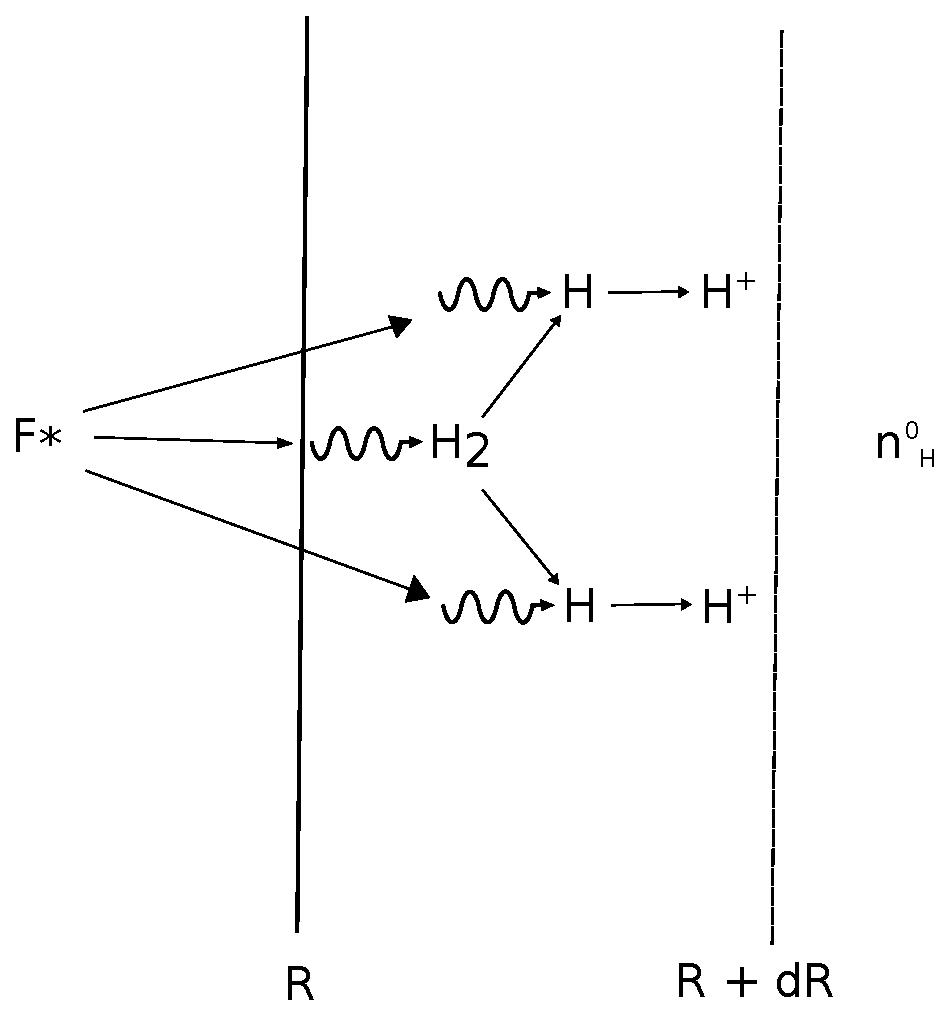
\includegraphics[width=0.6\linewidth]{./Figures/ionization}
%  \caption{Representación de la primera expansión del frente de ionización de una región $HII$ con densidad numérica del hidrógeno $n^0_H$. De cada tres fotones ionizantes que cruzan el frente en R, uno disocia una molécula de hidrógeno y los otros dos ionizan los átomos resultantes \citep{Stahler:2004}}
%  \label{fig:ionization}
%\end{figure}


%Estamos asumiendo que el flujo tanto de fotones con energías de $E\geq 14.7\mathrm{~eV}$ y $E\geq 13.6\mathrm{~eV}$ es prácticamente el mismo.

%Ahora consideremos las recombinaciones: el número total de recombinaciones que llevan a niveles tales que $n \geq 2$ dentro de una esfera de radio $R$ es $\frac{4\pi}{3}\left(n^0_H\right)^2\alpha'_{rec}R^3$. Si el balance de ionización aun se mantiene, entonces el número de ionizaciones por unidad de tiempo es igual a la tasa de recombinaciones más los fotones que logran atravesar el frente de ionización por unidad de tiempo que es $4\pi R^2 F_*$. Entonces:

%\begin{align}
%  \Nio_* = 4\pi R^2 F_* + \frac{4\pi}{3}\left(n^0_H\right)^2\alpha'_{rec}R^3
%\end{align}

%Resolvemos para $F_*$ y encontramos que:

%\begin{align}
%  F_* &= \frac{\Nio_*}{4\pi R^2} - \frac{\left(n^0_H\right)^2\alpha'_{rec} R}{3} \\
%  \implies \frac{dR}{dt} &= \frac{\Nio_*}{6\pi n^0_H R^2} - \frac{2n^0_H \alpha'_{rec} R}{9} \label{eq:1-expansion-eq} 
%\end{align}

%Definimos los siguientes parámetros adimensionales $\lambda \equiv R/R_s$ y $\tau \equiv t/t_{rec}$, donde $t_{rec} = \frac{1}{n^0_H \alpha'_{rec}}$ es el tiempo medio de recombinación del hidrógeno, que es del órden de $60\mathrm{~yr}$ con los valores de $n^0_H$ y $\alpha'_{rec}$ utilizados en esta sección. Y con esto la ecuación (\ref{eq:1-expansion-eq}) se escribe como sigue:

%\begin{align}
%  \frac{d\lambda}{d\tau} = \frac{2}{9}\left(\lambda^{-2} - \lambda\right) \label{eq:d-lambda-tau}
%\end{align}

%Resolvemos por el método de separación de variables y aplicamos la condición inicial $\lambda(0) = 0$ y obtenemos lo siguiente:

El radio de la región HII durante la primera expansión se comporta siguiendo la siguiente expresión:
\begin{align}
  \lambda(\tau) = \left[1 - \exp\left(-\frac{2}{3}\tau\right)\right]^{1/3} \label{eq:lambda-tau}
\end{align}

Donde $\lambda\equiv R/R_s$, $\tau\equiv t/t_{rec}$ y $t_{rec}\equiv \frac{1}{n^0_H \alpha'_{rec}}$ que es el tiempo medio de recombinación del hidrógeno.

De la ecuación (\ref{eq:lambda-tau}) vemos que cuando han pasado una y media veces del tiempo de recombinación,  la región $HII$ se ha expandido alrededor del $86\mathrm{\%}$ del radio de Strömgren, y aunque la expansión se va descelerando constantemente, ya es de una extensión considerable.

La velocidad del sonido en el gas ionizado con temperatura de $\sim 10^4\mathrm{K}$ es de $a_{II}\sim 10\mathrm{km~s^{-1}}$, si comparamos esta velocidad con la media de la velocidad del frente de ionización, por ejemplo, en el intervalo $0< \tau < \frac{3}{2}$, en el que ya comprobamos que el frente de ionización casi alcanza el radio de Strömgren, encontramos lo siguiente:

\begin{align}
  \bar{v}_{IF} = \frac{R_s}{t_{rec}}\frac{1}{\frac{3}{2}- 0}\int^{\frac{3}{2}}_0 \frac{d\lambda}{d\tau}~d\tau = \frac{2R_s}{3t_{rec}}\lambda\left(3/2\right)
\end{align}

Con los valores típicos adoptados en esta sección obtenemos que:

\begin{align}
  \bar{v}_{IF}\simeq 135\mathrm{~km~s^{-1}}\left(\frac{\Nio_*}{10^{49}\mathrm{~s^{-1}}}\right)^{1/3}\left(n_{H_2}\right)^{-2/3}
\end{align}

%Dado que la velocidad media del IF es mucho mayor que la del sonido del gas ionizado, entonces es razonable asumir que la densidad del gas ionizado es igual a la del gas neutro dado que la densidad del gas no tiene tiempo de reajustarse después de ser ionizado. Sin embargo, la presión sí se vuelve mucho mayor en el gas ionizado que en el gas de la nube circundante, tanto que incluso el frente de ionización es precedido por una onda de choque, dejando una delgada capa de gas neutro entre el frente de ionización y la onda de choque (ver figura \ref{fig:second-expansion}), y este gas empieza a generar una segunda expansión más lenta que la primera, que provoca que la densidad del gas ionizado disminuya, hasta que llega a un equilibrio de presión con el gas neutro circundante.

%\begin{figure}
%  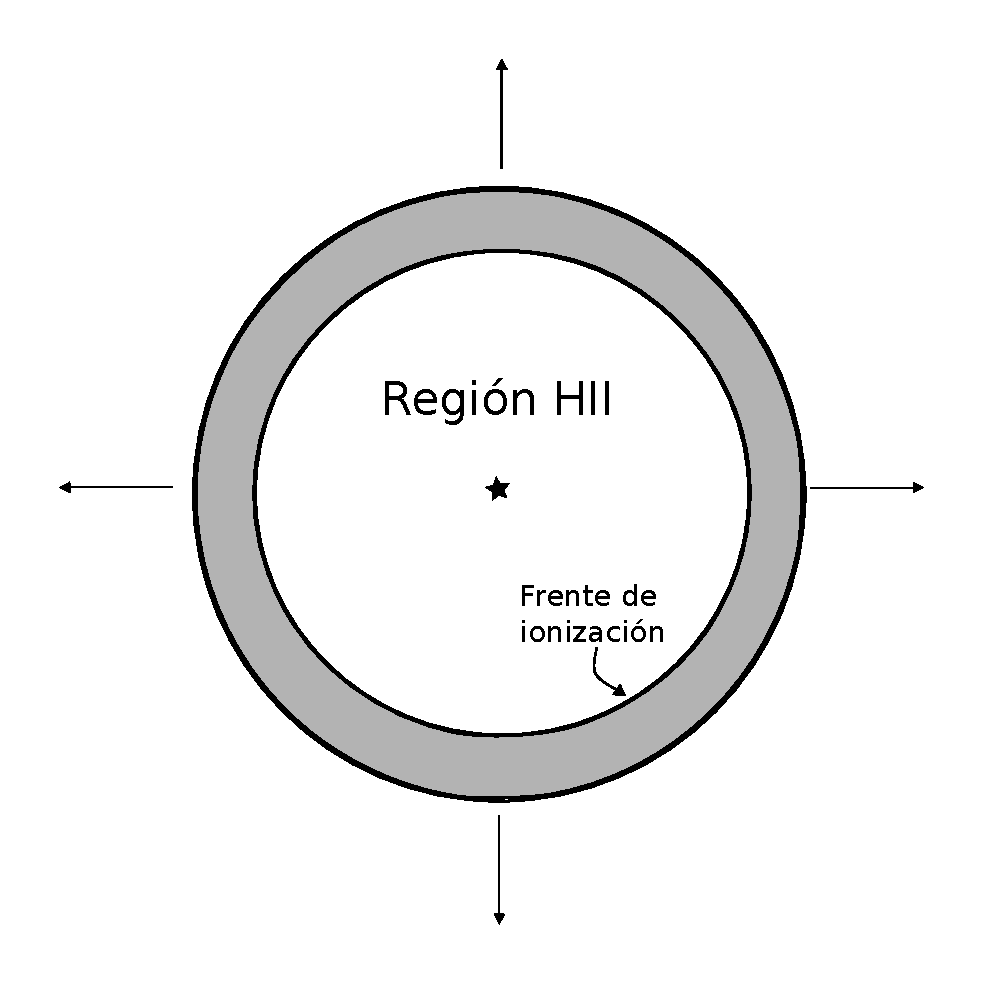
\includegraphics[width=0.6\linewidth]{./Figures/second-expansion}
%  \caption{Representación esquemática de la segunda expansión de la región HII: Dado que la diferencia de presiones entre el gas neutro e ionizado es muy grande, se forma una onda de choque que precede al frente de ionización, dejando una capa de gas neutro entre ambas (región sombreada). Por esta misma diferencia de presiones, esta capa se expande hasta que se logre el equilibrio de presión.}
%  \label{fig:second-expansion}
%\end{figure}


%Para encontrar el comportamiento de la segunda expansión, nos basamos en que el enfriamiento pos choque es muy eficiente y por tanto el choque puede ser considerado isotérmico. En este caso, el equilibrio de presiones entre la región HII y la capa de gas neutro viene dada por:

%\begin{align}
%  n^1_H a^2_1 = n^0_H\left(\frac{dR}{dt}\right)^2 \label{eq:sec-exp-P-equililibrium}
%\end{align}
%Donde $n^1_H$ es la densidad numérica del gas ionizado, $a_1$ la velocidad del sonido del gas ionizado y $dR/dt$ es la velocidad a la que se expande la onda de choque.

%Ahora, casi todos los fotones ionizantes en esta etapa son consumidos en la región HII, de esta forma modificamos la ecuación (\ref{eq:stromgren}) como sigue:

%\begin{align}
%    R = \left[\frac{3\Nio_*}{4\pi\alpha'_{rec}(n^1_H)^2}\right]^{1/3} \label{eq:second-exp}
%\end{align}

%Combinando las ecuaciones (\ref{eq:sec-exp-P-equililibrium}, \ref{eq:second-exp}) encontramos la ecuación de movimiento de la segunda expansión:

%\begin{align}
%  \left(\frac{dR}{dt}\right)^2 = \frac{a^2_1}{n^0_H}\left[\frac{3\Nio_*}{4\pi\alpha'_{rec}R^3}\right]^{1/2} = a^2_1\left(\frac{R}{R_s}\right)^{-3/2} \label{eq:second-exp-motion}
%\end{align}

%De nuevo hacemos el cambio de variable $\lambda \equiv R/R_s$, pero en esta ocasión definiremos una nueva variable detiempo adimensional $\tau' \equiv a_1 t/R_s$, para que la ecuación (\ref{eq:second-exp-motion}) quede como sigue:

%\begin{align}
%  \frac{d\lambda}{d\tau'} = \lambda^{-3/4}
%\end{align}

%Integrando y tomando como condición inicial $\lambda(0) = 1$, puesto que la primera expansión es bastante rápida, encontramos que:
Para la segunda expansión encontramos lo siguiente:

\begin{align}
  \lambda = \left(1 + \frac{7\tau'}{4}\right)^{4/7}
\end{align}
Donde $\tau' \equiv a_1 \frac{t}{R_s}$ y $a_1$ es la velocidad del sonido del gas ionizado.

\subsection{Flujos de Champaña}
La segunda expansión lleva a que la región $HII$ se expanda dos órdenes de magnitud por encima del radio de Strömgen, pero el tiempo que toma alcanzar dichas dimensiones es tan largo que la estrella central muere antes de que la región $HII$ alcanze el equilibrio de presiones. Sin embargo, es más probable que el frente de ionización rebase el borde de la nube molecular donde se formó, y en este caso el gas ionizado altamente presurizado escapa directamente hacia el medio interestelar que lo rodea (que tiene una presión aún menor que la de la nube molecular), creando el \textit{Flujo de champaña}.

\subsection{Características de la emisión}


\includegraphics[width=0.1\linewidth]{./Figures/tux-development}